\section{Effect of Problem Domain Size and Precision} \label{sec:res-size}

\subsection{Change in X and Y Domain Size}

\begin{figure}
	% dat=pd.concat([large, medium, small])
% dat["rel"]=u.relmingroup(dat,by=u.col.size+u.col.stencil)
% fastest=u.groupmin(dat, by=u.col.problem+u.col.variant+u.col.storage)
	% u.barplot(fastest[fastest["unstructured"]&(fastest["size-z"]==64)&(fastest["stencil"]=="laplap")], cat=u.col.size, grp=u.col.variant, y="rel", tickrot=0)
	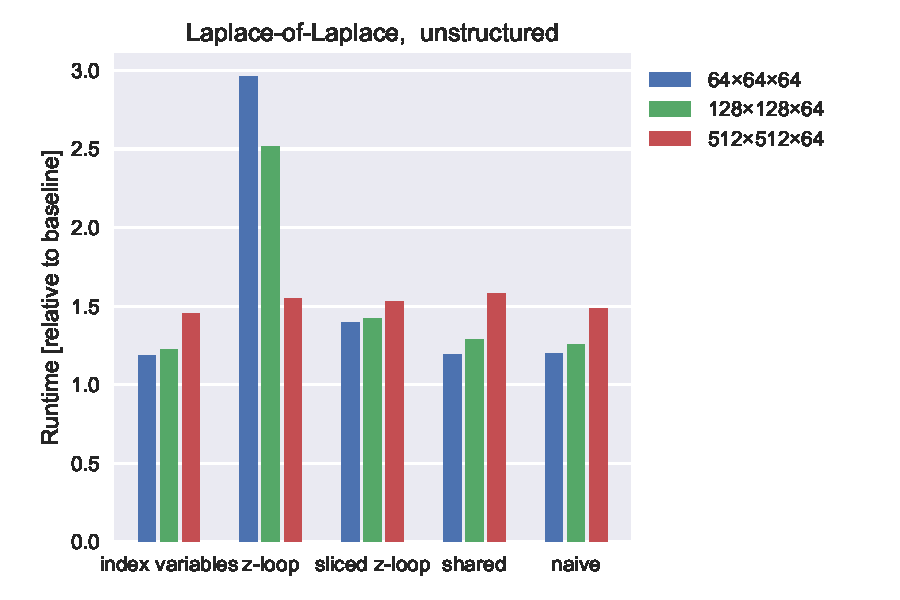
\includegraphics[scale=0.75]{variants-gridsizes.pdf}
	\caption{\label{fig:variants-gridsizes} Relative runtime of different variants of the Laplace-of-Laplace benchmark at different X-Y-sizes with respect to the fastest regular variant. For each bar, the fastest storage variant is considered (fastest of compression/chasing/z-curves). Baseline: fastest regular grid implementation.}
\end{figure}

We have evaluated combinations of grid storage and access variants for the three stencils on grids of X-Y size $64\times 64$ (small grid), $128\times 128$ (medium grid) and $512\times 512$ (large grid). Naturally, larger problem sizes lead to longer run times in all variants. More intrestingly however, increases in the X-Y-domain size affect the unstructured variants more negatively than the regular ones.

For small domains, the runtimes of unstructured variants are generally close to those of their regular counterparts. With increased domain size, there is an increase in the relative slowdown of the unstructured variant with respect to the fastest regular implementation. We assume this is due to cache sizes; while in smaller grids, entire neighborship tables and cell values remain cached, larger grids necessitate larger neighborship tables which cannot fit into the cache together with the cell values as a whole. Figure \ref{fig:variants-gridsizes} shows this trend for the Laplace-of-Laplace benchmark, but the same characteristics apply to the other stencils as well.

The \emph{z-loop} grid access variant is the only exception to the described charateristics. Its relative slowdown decreases for larger grid sizes. This is probably due to two reasons. First, the z-loop variants already suffer from low occupancy in large grids. In small grids, occupancy is even lower, not making use of the complete parallelism capabilities of the GPU. Second, in small grids, the neighborship table may be in cache in its entirety after one read. This allows subsequent neighborship table accesses to be practically free. This offsets the supposed optimization of the z-loop variant, which aims to reduce the number of reads of neighborship table entries. This optimization only begins to provide a benefit in large grids.

\subsection{Change in Z domain size}

\begin{figure}
	% dat = pd.read_csv("results/ultimate-reformat.csv")
	% dat["rel"] = u.relmingroup(dat, by=u.col.stencil+u.col.size)
	% u.lineplot(dat[(dat["stencil"]=="laplap")&(dat["variant"]=="idxvar")&dat["z-curves"]], x="size-z", y="rel")
% fig=u.plotdone(legend=0)
	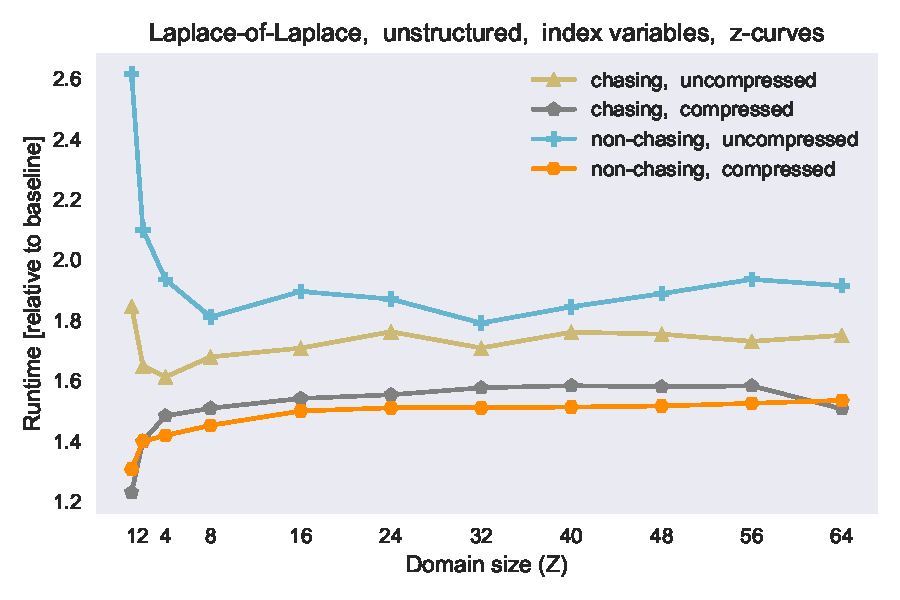
\includegraphics[scale=0.75]{laplap-idxvar-z-sizes.pdf}
	\caption{\label{fig:laplap-z-sizes} Relative slowdowns of the Laplace-of-Laplace stencil on unstructured grids of various Z-sizes. Baseline: fastest regular grid implementation.}
\end{figure}

Given a $512\times 512$ base grid, we benchmarked our stencils with various Z-sizes ranging from $1$ to $64$. We analyzed the cost of using an unstructured grid relative to a regular grid, and observe two main patterns. Which pattern the relative costs follow depends on the chosen grid storage. Figure \ref{fig:laplap-z-sizes} plots the relative slowdowns as a function of the Z-size for the \emph{laplap} stencil using the \emph{idxvar} access method. The plot is roughly representative of all other stencils and access methods. The observed patterns are as follows:

First, for uncompressed storage, the overhead decreases quickly for the first few Z-size steps, then fluctuates around some constant. This can be most clearly be seen in the \emph{non-chasing} stored grids. Second, when compression is used, the overhead increases in the first few Z-size steps, then also remains roughly constant.

These trends can be explained by two countering effects:

On one hand, the increased number of Z-levels obviously results in an increased total number of cells. In an unstructured grid, for each of those cells, some extra effort has to be made to determine the location of the cell's neighbors. We call this the \emph{once-per-cell cost}. This effect alone would lead to constant additional relative costs (linear additional absolute costs) with respect to the regular grid.

On the other hand, as our grids are regular in the Z-dimension, neighborship pointers can be re-used among threads operating on cells with the same X- and Y-coordinates. Let us call a set of cells with identical X- and Y-coordinates a \emph{pillar of cells}. If neighborship pointers are effectively reused, loading them is only a \emph{once-per-pillar} cost. No matter how many Z-levels there are in the grid, the first load of the neighborhip pointers remains a constant cost. As Z-size increases, this constant becomes vanishingly small in relation to the overall cost of the regular-grid computation. Thus, considering only the \emph{once-per-pillar} costs, performance should approach regular grid performance asymptotically for increasing Z. 

The observed relative overheads result from a combination of the two described effects (\emph{once-per-cell} and \emph{once-per-pillar} costs). In the uncompressed variants, the \emph{once-per-pillar costs} appear to dominate; thus, an increase in Z-size leads to better relative runtimes. One could say the ``investment'' of loading the neighborship pointers pays off once they can be reused more often (larger Z-sizes).

Our optimized access strategies aim to make explicit use of the \emph{once-per-pillar} nature of neighborship reads (\emph{shared}, \emph{z-loop} and \emph{z-loop-sliced}). Even the access strategies that do not explicitly exploit Z-regularity benefit from it if neighborship pointers happen to reside in caches (which they most likely will for adequate block sizes due to their frequency of use).  In the best-case scenario, all neighborship pointers are already in L1 cache (\emph{idxvar}), shared memory (\emph{shared} access strategy) or loaded into registers at the beginning of a loop (\emph{z-loop}) when a thread begins computation.

\subsection{Effect of Floating Point Precision}

We observed no significant differences in the relative slowdown when using single-precision floating point data types instead of double-precision data types. As expected, the absolute runtimes decrease with lower precision. This happens in the same proportions for both regular grid and unstructured grid implementations -- both are roughly $40\%$ faster than double-precision speeds.

As it appears to have no effect on the characteristics of our benchmarks, we consistently used double precision data types in all other experiments apart from this section.